\documentclass[a4paper,11pt]{article}
\usepackage[T1]{fontenc}
\usepackage[utf8]{inputenc}
\usepackage{lmodern}
\usepackage{amsmath}
\usepackage{amsfonts}
\usepackage{amssymb}
\usepackage{amsthm}
\usepackage{graphicx}
\usepackage{color}
\usepackage{url}
\usepackage{textcomp}
\DeclareMathOperator*{\argmax}{argmax}
\DeclareMathOperator*{\argmin}{argmin}

\title{Value Iteration}
\author{Joshua Tsang}
\date{\today}

\begin{document}

\maketitle
\tableofcontents

\section{Foundational Concepts}

It is instructive intially discuss the foundational concepts in Markov Decision Problems (MDP) and Reinforcement Learning (RL).  Consider the problem shown in Figure \ref{fig:1d-grid-world-problem-statement} where an agent is located in one of the grid positions.

\begin{figure}
    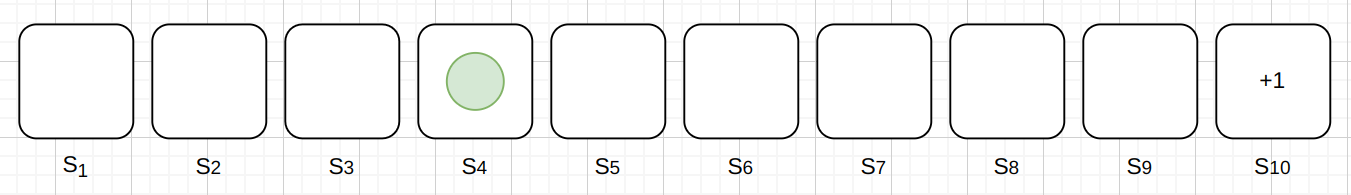
\includegraphics[width=\textwidth]{images/1d-grid-world-problem-statement.png}
    \caption{1D Grid World MDP with an assigned reward of $+1$ in state $s_{10}$.  The agent currently sits in state $s_4$ and the goal of the problem is for the agent to take actions to maximise its reward.}
    \label{fig:1d-grid-world-problem-statement}
\end{figure}


\begin{itemize}
    \item State Space and State: The finite State Space of a system is denoted $S$ where a state $s$ denotes a certain configuration of the system i.e. $s \in S$.  For example, in Figure \ref{fig:1d-grid-world-problem-statement} the agent is currently in state $s_4$, with the neighbouring states, $\{s'\}$, being $s_3$ and $s_5$.
    \item Actions: For each state, $s_i$, that the system resides in a set of available actions, $\{a_k\}$, can be taken that transition the system to another state, $s_j$.  For Figure \ref{fig:1d-grid-world-problem-statement} the available actions at state $s_4$ are \verb|(move left)| and \verb|(move right)|.  One could think of a graph where nodes are states and the edges are actions.
    \item Policy: A policy, denoted $\pi$, dictates the action to take for a given state.  It is often written as a function $\pi(s, a)$ where it is formally defined as:
    \begin{equation} \label{eqn:policy_formal_definition}
        \pi(s,a) = P(a=a|s=s)
    \end{equation}
    which is the probability of take action $a$ given the system is in state $s$.  As a foreshadow, policy functions are often expressed as an $\argmin_a$ as follows:
    \begin{equation} \label{eqn:value_iteration_foreshadow}
        \pi(s,a) = \argmax_a Q(s, a)
    \end{equation}
    i.e. an $\argmax$ over the available actions which returns the argument (action) that returns the maximum value for the quality function $Q$ (defined later).
    \item Reward: 
  \end{itemize}

\section{Value Iteration}

Defining the quality function as:
\begin{equation} \label{eqn:quality_function_Q}
    Q(s,a) = \sum_{s'} P(s'|s,a) \left[ R(s',s,a) + \gamma V(s') \right]
\end{equation}
where $s'$ are the neighbouring states to the current state, $s$.



\begin{figure}
    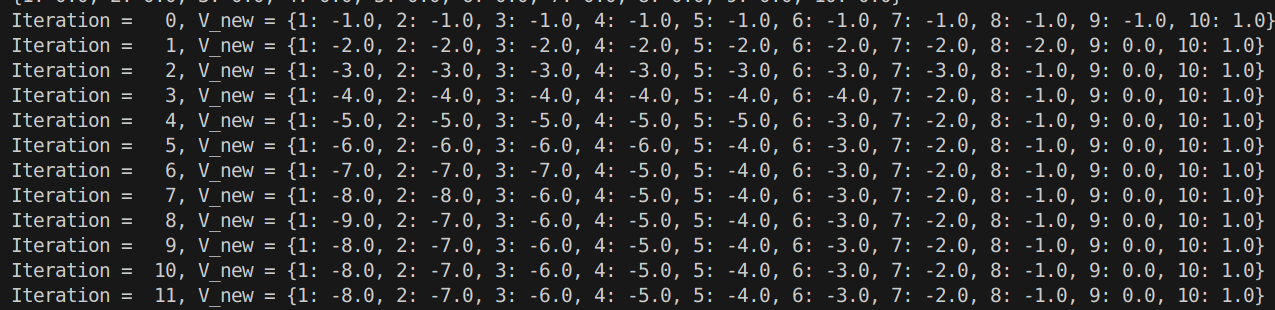
\includegraphics[width=\textwidth]{images/iters-of-value-iteration-1d-grid-world-code-output.png}
    \caption{Iterations of the value iteration algorithm.}
    \label{fig:iters-of-value-iteration-1d-grid-world-code-output}
\end{figure}

\end{document}